\documentclass[11pt,a4paper]{article}
\usepackage{amsmath,amssymb}
\usepackage{tikz}
\usetikzlibrary{bayesnet,arrows.meta,positioning,calc,graphs,matrix,automata,fit,backgrounds,shapes}

% Example of different automatic graph layout approaches

\title{Automatic Graph Layout Options for Directed Graphical Models in LaTeX}
\date{\today}

\begin{document}
\maketitle

\section{Option 1: Using tikz-bayesnet Package}

The \texttt{tikz-bayesnet} package provides automatic styling for Bayesian networks:

\begin{center}
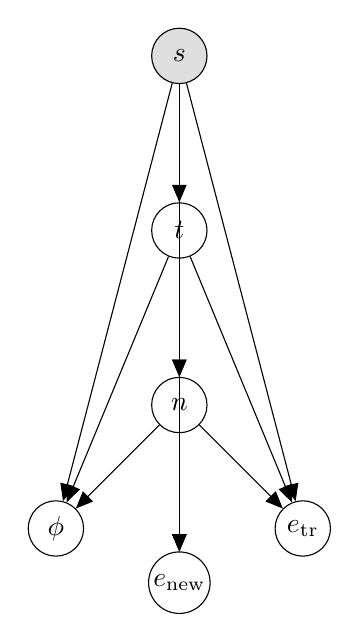
\begin{tikzpicture}
  % Define nodes using the bayesnet macros
  \node[obs] (s) {$s$};
  \node[latent, below=1.5 of s] (t) {$t$};
  \node[latent, below=1.5 of t] (n) {$n$};
  \node[latent, below left=1.5 of n] (phi) {$\phi$};
  \node[latent, below=1.5 of n] (new) {$e_{\text{new}}$};
  \node[latent, below right=1.5 of n] (trans) {$e_{\text{tr}}$};

  % Edges
  \edge{s}{t,n,phi,new,trans}
  \edge{t}{n,phi,new,trans}
  \edge{n}{phi,new,trans}
\end{tikzpicture}
\end{center}

\section{Option 2: Using TikZ Matrix for Grid Layout}

Automatic grid alignment using matrix:

\begin{center}
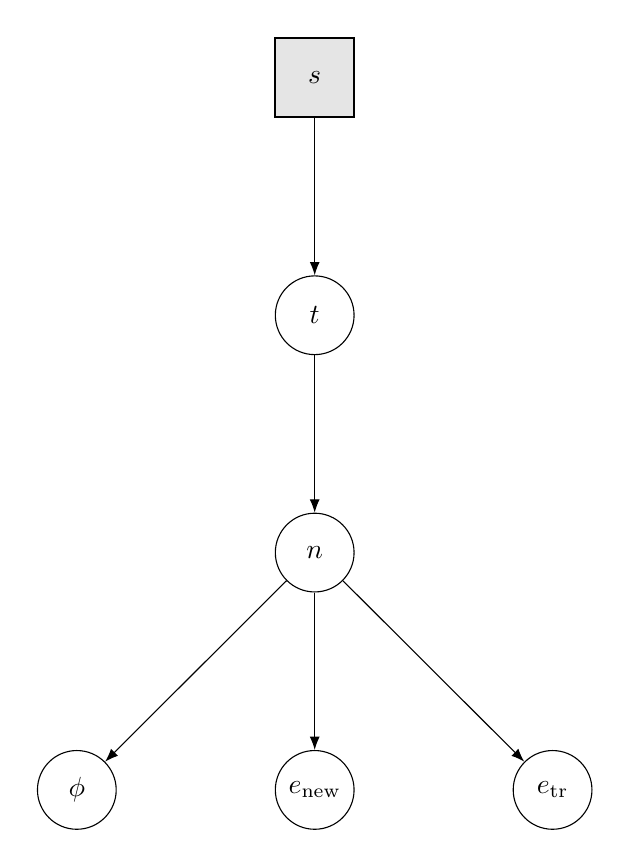
\begin{tikzpicture}[
  latent/.style={circle, draw, minimum size=1cm},
  obs/.style={rectangle, draw, thick, minimum size=1cm, fill=gray!20},
  every edge/.style={draw, -{Latex}}
]
  \matrix[row sep=2cm, column sep=2cm] {
    & \node[obs] (s) {$s$}; & \\
    & \node[latent] (t) {$t$}; & \\
    & \node[latent] (n) {$n$}; & \\
    \node[latent] (phi) {$\phi$}; &
    \node[latent] (new) {$e_{\text{new}}$}; &
    \node[latent] (trans) {$e_{\text{tr}}$}; \\
  };

  \path[every edge]
    (s) edge (t)
    (t) edge (n)
    (n) edge (phi)
    (n) edge (new)
    (n) edge (trans);
\end{tikzpicture}
\end{center}

\section{Option 3: Using Graph Drawing Library (Requires LuaLaTeX)}

For automatic layout algorithms, compile with \texttt{lualatex}:

\begin{verbatim}
\begin{tikzpicture}[>={Stealth}]
  \graph[layered layout, sibling distance=3cm, level distance=2cm] {
    s [as={$s$}, draw, rectangle, fill=gray!20];
    t [as={$t$}, draw, circle];
    n [as={$n$}, draw, circle];
    phi [as={$\phi$}, draw, circle];
    new [as={$e_{\text{new}}$}, draw, circle];
    trans [as={$e_{\text{tr}}$}, draw, circle];

    s -> {t, n, phi, new, trans};
    t -> {n, phi, new, trans};
    n -> {phi, new, trans};
  };
\end{tikzpicture}
\end{verbatim}

\section{Option 4: Using Python + GraphViz/NetworkX}

You can generate the graph programmatically and include it:

\begin{verbatim}
# Python code
import matplotlib.pyplot as plt
import networkx as nx
from networkx.drawing.nx_agraph import graphviz_layout

G = nx.DiGraph()
G.add_edges_from([
    ('s', 't'), ('s', 'n'), ('s', 'phi'), ('s', 'e_new'), ('s', 'e_tr'),
    ('t', 'n'), ('t', 'phi'), ('t', 'e_new'), ('t', 'e_tr'),
    ('n', 'phi'), ('n', 'e_new'), ('n', 'e_tr')
])

pos = graphviz_layout(G, prog='dot')
nx.draw(G, pos, with_labels=True, node_color='lightblue',
        node_size=1500, font_size=16, arrows=True)
plt.savefig('graphical_model.pdf', format='pdf')
\end{verbatim}

Then include with: \verb|\includegraphics{graphical_model.pdf}|

\section{Option 5: Using tikz-dependency for Hierarchical Layout}

\begin{center}
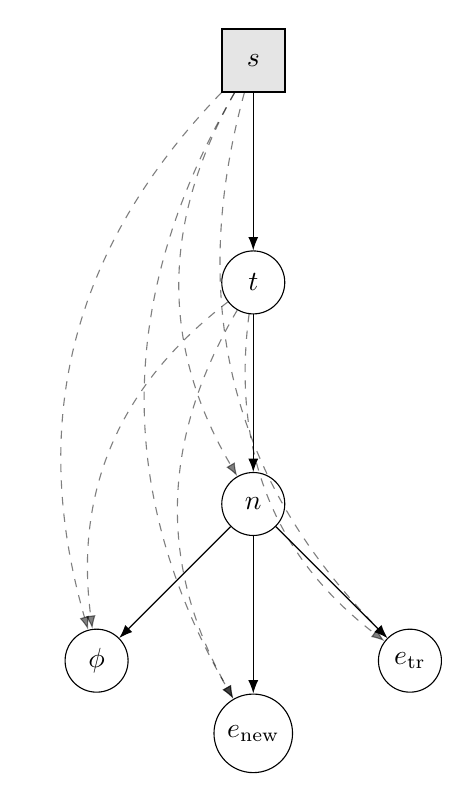
\begin{tikzpicture}[
  node distance=2cm,
  state/.style={rectangle, draw, thick, fill=gray!20, minimum size=0.8cm},
  var/.style={circle, draw, minimum size=0.8cm}
]
  % Use chain positioning for automatic flow
  \begin{scope}[start chain=going below, every node/.append style={on chain}]
    \node[state] (s) {$s$};
    \node[var] (t) {$t$};
    \node[var] (n) {$n$};
  \end{scope}

  % Place bottom nodes using relative positioning
  \node[var] (phi) [below left=of n] {$\phi$};
  \node[var] (new) [below=of n] {$e_{\text{new}}$};
  \node[var] (trans) [below right=of n] {$e_{\text{tr}}$};

  % Automatic edge routing
  \foreach \from/\to in {s/t, t/n, n/phi, n/new, n/trans}
    \draw[-{Latex}] (\from) -- (\to);

  % Skip connections with automatic routing
  \foreach \from/\to in {s/n, s/phi, s/new, s/trans, t/phi, t/new, t/trans}
    \draw[-{Latex}, dashed, opacity=0.5] (\from) to[bend right] (\to);
\end{tikzpicture}
\end{center}

\section{Option 6: Define Reusable Styles}

Create a command for consistent graphical models:

\begin{verbatim}
\newcommand{\drawBN}[2]{
  \begin{tikzpicture}[
    bn/.cd,
    latent/.style={circle, draw, minimum size=8mm, bn/label=#1},
    obs/.style={rectangle, draw, thick, fill=gray!20, minimum size=8mm},
    edge/.style={-{Latex}, thick},
    #2
  ]
}
\end{verbatim}

\section{Option 7: Using dot2tex}

You can write in DOT language and convert:

\begin{verbatim}
digraph G {
  rankdir=TB;
  node [shape=circle];
  s [shape=box, style=filled, fillcolor=gray];

  s -> t;
  s -> n;
  s -> phi;
  s -> "e_new";
  s -> "e_tr";
  t -> n;
  t -> phi;
  t -> "e_new";
  t -> "e_tr";
  n -> phi;
  n -> "e_new";
  n -> "e_tr";
}
\end{verbatim}

Then convert: \texttt{dot2tex --format tikz graph.dot > graph.tex}

\section{Recommendations}

\begin{enumerate}
\item For simple Bayesian networks: Use \texttt{tikz-bayesnet}
\item For complex automatic layout: Use LuaLaTeX with graph drawing
\item For programmatic generation: Use Python + NetworkX
\item For reusable components: Define custom TikZ styles
\item For very complex graphs: Generate externally and include as PDF
\end{enumerate}

\end{document}